

Zur Verarbeitung der Sensorsignale wurden mehrere Software Lösungen entwickelt.\\

Zum einen wurde eine Lösung zur Live Anzeige der Sensordaten und zum anderen zur Speicherung der Daten entwickelt. Die Software zur Speicherung kam in der durchgeführten Messreihe jedoch nicht zur Anwendung.\\

\begin{figure}[h]
    \centering
\begin{minipage}[t]{0.9\textwidth}
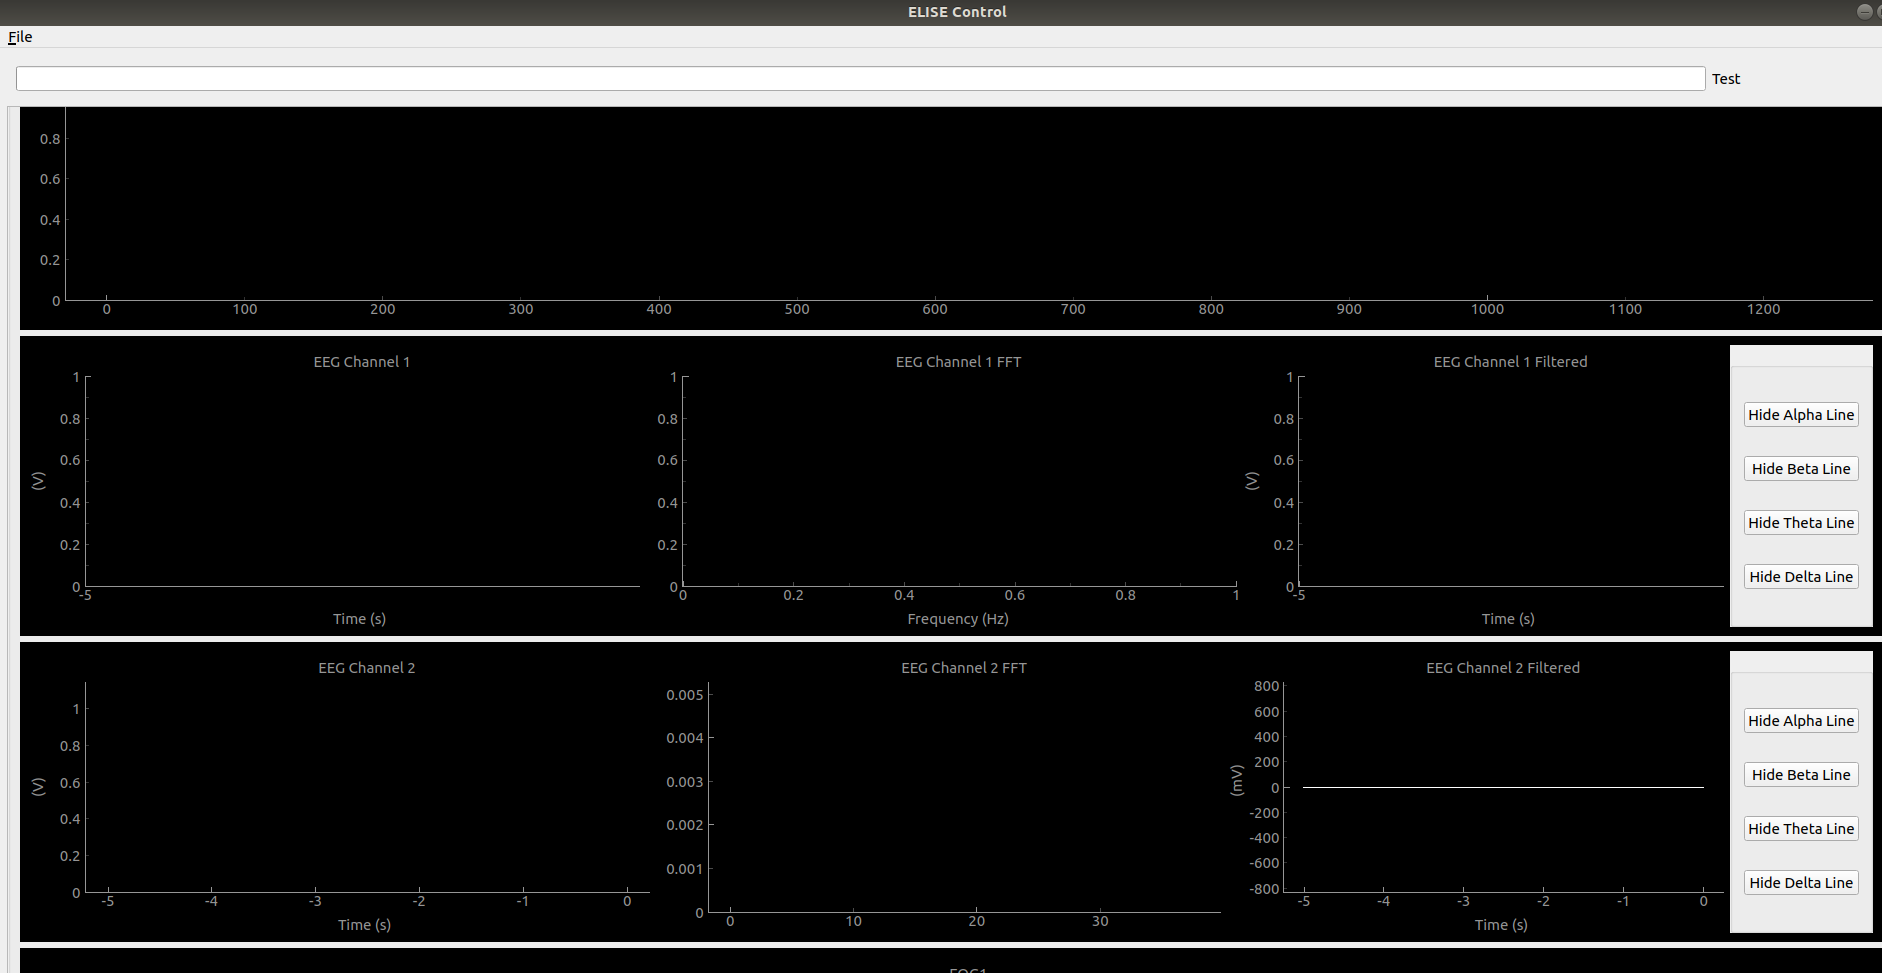
\includegraphics[width=\textwidth]{Images/screenshot_liveview.png}
\end{minipage}
    \caption{Software zur Anzeige der Sensordaten}
    \label{fig:screen_sensor}
\end{figure}

Die Software zur Live Anzeige empfängt die per UDP ausgesandten Daten. Da diese immer in Blöcken von 75 Datenpunkten gesendet werden, werden die empfangenen Daten zunächst in einem Buffer zwischengespeichert. Dieser Buffer emittiert dann einen kontinuierlichen Datenstrom mit einer Samplerate von 250 Samples je Sekunde. Werden keine neuen Daten empfangen emittiert der Buffer Nullwerte, ebenfalls mit einer Samplerate von 250 Samples je Sekunde.  Dieser kontinuierliche Datenstrom wird nun in den Viewbuffer eingelesen der die letzten 5 Sekunden an Daten vorhält (d.h. 1250 Datenwerte). Dieser Viewbuffer wird mit einer Framerate von 25 Frames pro Sekunde gerendert. Dies ermöglicht eine flüssige aber auch performante Anzeige der Datenwerte. Durch den Zwischenbuffer in dem die Daten eingelesen werden entsteht ein minimales Delay von ungefähr 100 ms zwischen dem Auftreten eines Ereignisses und der Anzeige am Display. Dies ist in der praktischen Anwendung vernachlässigbar. \\

Angezeigt werden neben den Rohdaten für jeden Kanal auch die Fouriertransformationen für die EEG und EOG Kanäle. Für die EEG Kanäle beteht weiterhin die Möglichkeit nach den einzelnen Komponenten, also Alpha, Beta, Delta und Theta Wellen, zu filtern und nur diese jeweils anzuzeigen. Alle Werte werden von ihrem übermittelten Zahlenwert umgerechnet in den korrespondierenden Millivolt Wert beziehungsweise in Grad Celcsius bei der Temperatur. Ebenfalls erfolgt eine Filterung der Werte softwareseitig. So wird standardmäßig für GSR, EOG und EEG ein Bandpassfilter angewendet, der den Frequenzraum auf ein für das Biosignal sinnvolle Maß beschneidet. 

\begin{figure}[h]
    \centering
\begin{minipage}[t]{0.9\textwidth}
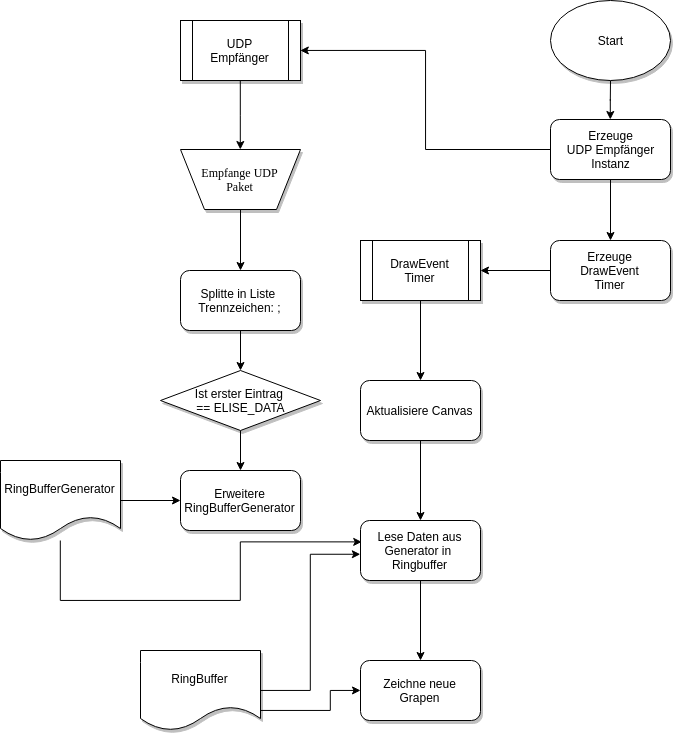
\includegraphics[width=\textwidth]{Images/ablauf_anzeige.png}
\end{minipage}
    \caption{Schematischer Ablauf der Anzeige}
    \label{fig:schema_anzeige}
\end{figure}

